\documentclass[Master,ngerman,UKenglish]{scrbook}
%------------------------------------------------------------------------------
% This file contains a skeleton thesis for
% a Physics or Astronomy Institute in the University of Bonn

% Specify the thesis type as an option: PhD, Master, Diplom, Bachelor
% Specify the thesis stage as an option: Draft (default), Submit, Final, PILibrary

% Specify the language(s) in the class and then use babel.
% If you need more than one language, give the default language last,
% e.g. ngerman,UKenglish for a thesis in British (UK) English where you want
% to be able to set the language to German for some part of it.

%------------------------------------------------------------------------------
% Pass TeX Live version to the package
% Use command pdflatex --version to find out which version you are running
% Add option backref=false when your thesis is ready to turn off back-referencing
% in your bibliography
\usepackage[texlive=2014,astrobib]{ubonn-thesis}
% Adjustments to standard biblatex style
\usepackage{ubonn-biblatex}

% Glossary package
% \usepackage[acronym,toc,nosuper]{glossaries}
% TikZ packages and libraries
% \usepackage{tikz}
% \usepackage{tikz-3dplot}
% \usepackage{pgfplots}
% \usetikzlibrary{positioning,shapes,arrows}
% \usetikzlibrary{decorations.pathmorphing}
% \usetikzlibrary{decorations.markings}
\usepackage{thesis_defs}

%------------------------------------------------------------------------------
% Instead of colouring  links, cites, table of contents etc.
% put them in a coloured box for the screen version.
% This is probably a good idea when you print your thesis.
% \hypersetup{colorlinks=false,
%   linkbordercolor=blue,citebordercolor=magenta,urlbordercolor=darkgreen
% }

%------------------------------------------------------------------------------
% When writing your thesis it is often helpful to have the date and
% time in the output file. Comment this out for the final version.
\ifoot[\today{} \thistime]{\today{} \thistime}

% In order to check if your labels are referenced try the refcheck package
% \usepackage{refcheck}

%------------------------------------------------------------------------------
% biblatex is included by ubonn-thesis. Look there for the settings used.
% See the options for settings that can be changed easily.
% For further changes copy the \RequirePackage[...]{biblatex} here
% and include ubonn-thesis with the option biblatex=false.

% Specify the bibliography files here and not at the end!
% Use standard_refs-bibtex if you use bibtex or bibtex8
% and standard_refs-biber  if you use biber
\addbibresource{thesis_refs.bib}
\addbibresource{../refs/standard_refs-biber.bib}

% You can include the following lines if you want to shorten your
% bibliography by not including url fields
% \AtEveryBibitem{\clearfield{url}}
% \AtEveryCitekey{\clearfield{url}}

%------------------------------------------------------------------------------
% The following definitions are used to produce the title pages
% needed at various stages
\newcommand{\thesistitle}{Title of the Thesis}
\newcommand*{\thesisauthor}{Author's name}
\newcommand*{\thesistown}{Place of birth}
\renewcommand*{\InstituteName}{\AIFA}
\renewcommand*{\inInstitute}{\inAIFA}
\renewcommand*{\InstituteAddress}{\PIaddress}
% Adjust \thesisreferee...text depending on male/female referee
\newcommand*{\thesisrefereeonetext}{1.\ Gutachter}
\newcommand*{\thesisrefereeone}{Prof.\ Dr.\ John Smith}
\newcommand*{\thesisrefereetwotext}{2.\ Gutachterin}
\newcommand*{\thesisrefereetwo}{Prof.\ Dr.\ Anne Jones}
% Date when thesis was submitted (Master/Diplom)
% Year or Month, Year when thesis was submitted (PhD)
\newcommand*{\thesissubmit}{XX.YY.2016}
% \newcommand*{\thesissubmit}{Month 2016}
% Date of thesis examination (PhD)
\newcommand*{\thesispromotion}{XX.YY.2016}
% Month and year of the final printed version of the thesis
\newcommand*{\thesismonth}{MMM}
\newcommand*{\thesisyear}{2016}
\newcommand*{\thesisnumber}{BONN-IR-2016-XXX}

%------------------------------------------------------------------------------
% The abstract is only needed for the printed version and should be in
% English regardless of the language of the thesis
\newcommand{\thesisabstract}{%
  \begin{otherlanguage}{UKenglish}
    This is your thesis abstract. It may be in a language that is
    different from the rest of your thesis.
  \end{otherlanguage}
}

%------------------------------------------------------------------------------
% \includeonly can be used to select which chapters you want to process
% A simple \include command just inserts a \clearpage before and after the file
% Note that \includeonly can be quite picky! Do not forget to put a
% comma after the filename, otherwise it will simply be ignored!
% \includeonly{%
%   thesis_intro,
%   thesis_appendix,
%   thesis_acknowledge
% }

%------------------------------------------------------------------------------
% Give a list of directories where figures can be found. Do not leave
% any spaces in the list and end the directory name with a /
\graphicspath{%
  {../figs/}%
  {../figs/cover/}%
  {../figs/graphics/}%
  {../feynmf/}%
}

%------------------------------------------------------------------------------
% Make a glossary and a list of acronyms
% \makeglossaries

% Glossary entries
% \input{thesis_glossary}

% Draft version - add the word DRAFT on the cover pages
\ifthenelse{\equal{\ThesisVersion}{Draft}}{%
  \usepackage{background}
  \ifthenelse{\texlive < 2013}{%
    \SetBgContents{DRAFT}
    \SetBgColor{blue!30}
  }{%
    \backgroundsetup{contents=DRAFT, color=blue!30}
  }
}

%------------------------------------------------------------------------------
\begin{document}

% Cover page of thesis - this is only needed for the printed final
% version to be submitted to the department library
% Do not use this page for thesis submission to the Prüfungsamt or Promotionsbüro!
\ifthenelse{\equal{\ThesisVersion}{PILibrary}}{%
  \typeout{Document \jobname, Info: PI library version of thesis}
  \input{../cover/\ThesisType_Cover}
}{}

% Start counting pages from the title page
\frontmatter
% Dedication has to come before \maketitle
% \dedication{For ...}

% Select the correct title page(s)
\ifthenelse{\equal{\ThesisType}{Unknown}}{%
  \typeout{Document \jobname, Error: Unknown thesis type - no title page printed}
}{%
  % Bachelor thesis only has one title page
  \ifthenelse{\equal{\ThesisType}{Bachelor}}{%
    \typeout{Document \jobname, Info: Bachelor thesis}
    \input{../cover/\ThesisType_Title}
  }{%
    \ifthenelse{\equal{\ThesisVersion}{Final} \OR \equal{\ThesisVersion}{PILibrary}}{%
      % Final and PI library versions
      \typeout{Document \jobname, Info: Final version of a \ThesisType  thesis}
      \input{../cover/\ThesisType_Final_Title}
    }{% Submission and draft versions
      \input{../cover/\ThesisType_Submit_Title}
      \typeout{Document \jobname, Info: Draft/submission version of a \ThesisType  thesis}
    }
  }
}

\pagestyle{scrplain}

%------------------------------------------------------------------------------
% You can add your acknowledgements here - don't forget to also add
% them to \includeonly above
%------------------------------------------------------------------------------
\chapter{Acknowledgements}
\label{sec:ack}
%------------------------------------------------------------------------------

This thesis would not have been possible without the help, guidance and support
of many people. Therefore, I would like to thank:
\begin{itemize}
\item Prof.\ Dr.\ Jochen Dingfelder for giving me the opportunity to write my
  thesis in his working group and for his continued support.

\item Prof.\ Dr.\ Klaus Desch for his willingness to co-examine my thesis.

\item Dr.\ William Davey for his excellent supervision, guidance and the many
  fruitful discussions.

\item Benedict Winter for his valuable advice and him sharing his vast
  knowledge of physics with me.

\item My (past) office colleagues Verena Muckhoff, Jan Heinrichs, and Christos
  Vergis for the enjoyable office atmosphere.

\item All of my colleagues in the working group of Prof.\ Dingfelder.

\item My family for providing me with support and stability during my studies.

\end{itemize}



%%% Local Variables:
%%% mode: latex
%%% TeX-master: "mythesis"
%%% End:


\tableofcontents

\mainmatter
\pagestyle{scrheadings}

% Turn off DRAFT for the following pages
\ifthenelse{\equal{\ThesisVersion}{Draft}}{%
  \ifthenelse{\texlive < 2013}{%
    \SetBgContents{}
  }{%
    \backgroundsetup{contents={}}
  }
}{}

%------------------------------------------------------------------------------
% Add your chapters here - don't forget to also add them to \includeonly above
\chapter{Introduction}
\label{sec:intro}

Outline of the thesis:

\section{Introduction}

\begin{itemize}
\item LHC \& Experiments
  \begin{itemize}
  \item Discoveries / Measurements

  \item Past: Run-I, Present: Run-II, Future: HL-LHC \& Challenges
  \end{itemize}

\item $\tau$-Leptons
  \begin{itemize}
  \item Importance (Fermionic coupling of Higgs, Higgs CP, Exotics $Z^\prime$,
    $W^\prime$, Heavy Higgs, SUSY)
  \item $\tau$-decay (hadronic branching fraction, decay modes)
  \item Jets faking taus (necessity of identification algorithms)
  \item Classification of $\tau$ decay modes (motivation)
  \end{itemize}

\item Overview of the thesis structure (one bullet point per chapter).
\end{itemize}

\section{Theoretical Background}

\begin{itemize}
\item The Standard Model
  \begin{itemize}
  \item Features \& Successes

  \item Challenges (neutrino masses, dark matter, matter-antimatter asymmetry,
    gravitation, number of parameters, hierarchy problem, \ldots)

  \item Beyond the Standard Model (SUSY -- preferred coupling to down-type
    fermions for large $\tan\beta$ \textrightarrow $\tau$-leptons)
  \end{itemize}

\item Weak Interaction
\begin{itemize}
\item ?
\end{itemize}

\item Strong Interaction
\begin{itemize}
\item ?
\item Confinement \& Hadronization
\item Quark \& Gluon initiated jets
\end{itemize}

\item $\tau$-Leptons
\begin{itemize}
\item Discovery

\item Properties (mass \textrightarrow lep \& had, mean life time
  \textrightarrow no direct detection)

\item Hadronically Decaying $\tau$-Leptons
  \begin{itemize}
  \item Feynman Diagram, Decay Modes (interm. resonances) \& Branching Ratios
  \item Detector signature ($\pi^0$ ($\gamma \gamma$ / $\mathrm{e}^+
    \mathrm{e}^- \gamma$), $\pi^\pm$ ($\mathrm{K}^\pm$), $\nu_\tau$)
  \item Jets faking taus
  \item
  \end{itemize}

\item $\tau$ Physics
  \begin{itemize}
  \item $\mathrm{Z} \rightarrow \tau \tau$ (background for H$\tau \tau$ and
    useful for performance measurements using tag-and-probe -- semileptonic
    decays)

  \item $\mathrm{H} \rightarrow \tau \tau$ (one of two channels to measure
    the fermionic coupling -- $b \bar{b}$ plagued by multijet background,
    Higgs CP)

  \item MSSM Higgs (potentially high branching fraction to $\tau$-leptons)

  \item $\mathrm{Z}^\prime$ could preferentially decay into third-generation
    fermions (lepton universality not required).

  \item $\mathrm{W}^\prime$ models with preferential coupling to third-gen.
  \end{itemize}
\end{itemize}

\end{itemize}

\section{Machine Learning (worthy of own chapter?)}

\begin{itemize}
\item Own chapter describing the machine learning methods used or include into
  \textit{Theoretical Background}? Alternatively include theory section where
  needed (e.g. have one for the BDT-based studies explaining BDTs [short] and
  one for the RNN studies [longer]).

\item Boosted Decision Trees
  \begin{itemize}
  \item Boosting: Adaptive Boosting $\alpha$, Gradient Boosting $\eta$
  \item Node splitting: Gini Index
  \item Hyperparameters: $N_\mathrm{Trees}$, $d_\mathrm{Tree}$,
  \end{itemize}

\item Neural Networks
  \begin{itemize}
  \item Basics -- focussed on forward pass (Densely connected layers, Activation)
  \item Training -- Weight initialization, Loss functions, Minibatch Gradient
    Descent, Cross-Validation (training, validation, test split)
  \item Recurrent Neural Networks (RNN Equations, Vanishing Gradient Problem,
    Physics Motivation)
  \item Long Short-Term Memory \cite{lstm} (LSTM Equations)
  \item Technical setup (Keras, theano)
  \end{itemize}
\end{itemize}

\section{ATLAS Experiment and the LHC}

\begin{itemize}
\item LHC (brief)

\item ATLAS
  \begin{itemize}
  \item Overview (Design goals) \\
    brief: Beam Line, Inner Detector \& Solenoid, Calorimeter, Muon System \&
    Toroid, Trigger

  \item Nomenclature (Coordinate system, Pseudorapidity, $\Delta R$)

  \item Inner detector / Tracker
    \begin{itemize}
    \item Pixel, IBL
    \item SCT
    \item TRT
    \item  Transverse Momentum Resolution, Vertex \& Secondary Vertex
      reconstruction, Impact Parameter Resolution, $\eta$-Coverage
    \end{itemize}

  \item Calorimeter
    \begin{itemize}
    \item Presampler, LAr (EM1 - EM3), Had (Tile, LAr)
    \item $\eta$-Coverage, Thickness $X_0$ / $\lambda$, Energy Resolution
      vs. $E$
    \item Topoclusters \& Cluster moments
    \end{itemize}

  \end{itemize}
\end{itemize}

\section{Reconstruction of Hadronically Decaying $\tau$-Leptons at ATLAS}

\begin{itemize}
\item anti-$k_\mathrm{t}$ Jets $R = 0.4$
\item Track Selection \& TJVA
\item MVA tracking
\item Energy \& Calibration
\item Tau-ID (does not fit in here)
\item Substructure Reconstruction (Decay Mode Classification)
\end{itemize}

\section{Identification of Hadronically Decaying $\tau$-Leptons (BDT part)}

\begin{itemize}
\item Features of hadronically decaying $\tau$-leptons vs. Quark/Gluon
  initiated jets

\item Samples
  \begin{itemize}
  \item Gammatautau (Polarization), Dijet JZ1W - JZ6W
  \item Reweighting
  \item Baseline selection ($\eta$, $p_\mathrm{T}$, truth-matching)
  \end{itemize}

\item BDT-based Studies
  \begin{itemize}
  \item Previous setup (incl. explanation \& plots of input variables)
  \item Hyperparameter optimization
    \begin{itemize}
    \item AdaBoost \textrightarrow GradBoost
    \item Grid Search
    \item XGBoost (?)
    \end{itemize}
  \item Variable correlations, importance (dropped variables) \& dependence with
    $p_\mathrm{T}$ (2D Hist), Variable Transformations (instead of cutting out
    outliers), Partial Dependence
  \item Working points (Gammatautau -- Ztautau)
  \item Performance on simulated data
  \item Impact of Quark / Gluon initiated jets on Tau-ID
  \end{itemize}

\end{itemize}

\section{Identification of Hadronically Decaying $\tau$-Leptons (NN-part)}

\begin{itemize}
\item Neural Network-based Studies
  \begin{itemize}
  \item MLP Tau-ID
  \item Track-RNN
    \begin{itemize}
    \item Architecture
    \item Input variables \& correlation with true class labels
    \item Validation loss vs. number of tracks
    \end{itemize}
  \item Cluster-RNN \& Potential rate-reduction at HLT
    \begin{itemize}
    \item Validation loss vs. number of clusters
    \item Input variables \& correlation with true class labels
    \end{itemize}
  \item Combined-RNN
  \end{itemize}
\end{itemize}

\section{Decay Mode Classification for Hadronically Decaying}

\begin{itemize}
\item Signature of the decay modes
\item Explain PFO
\item RNN
  \begin{itemize}
  \item Only PFOs
  \item PFOs + Extras
  \end{itemize}
\end{itemize}

\section{Conclusion}

\begin{itemize}
\item
\end{itemize}

\section{Appendix}

\begin{itemize}
\item MC Samples (Preprod, MC16A)
\end{itemize}

%%% Local Variables:
%%% mode: latex
%%% TeX-master: "mythesis"
%%% End:

% Uncomment the following command to get references per chapter.
% Put it inside the file or change \include to \input if you do not want the references
% on a separate page
\printbibliography[heading=subbibliography]

%------------------------------------------------------------------------------
% Use biblatex for the bibliography
% Add bibliography to Table of Contents
% Comment out this command if your references are printed for each chapter.
% \printbibliography[heading=bibintoc]

%------------------------------------------------------------------------------
% Include the following lines and comment out \printbibliography if
% you use BiBTeX for the bibliography.
% If you use biblatex package the files should be specified in the preamble.
% \KOMAoptions{toc=bibliography}
% {\raggedright
%   \bibliographystyle{../refs/atlasBibStyleWithTitle.bst}
%   % \bibliographystyle{unsrt}
%   \bibliography{./thesis_refs,../refs/standard_refs-bibtex}
% }

%------------------------------------------------------------------------------
\appendix
% \part*{Appendix}
% Add your appendices here - don't forget to also add them to \includeonly above
%------------------------------------------------------------------------------
\chapter{Auxiliary Information}
\label{sec:app}
%------------------------------------------------------------------------------

\begin{itemize}
\item MC Samples (Preprod, MC16A)
\item BDT ID studies \texttt{bdt\_tauid}
\item RNN ID studies \texttt{rnn\_tauid}
\item RNN Decay Mode studies \texttt{rnn\_decay\_mode\_classif}
\end{itemize}

\todo[inline]{Tables of layers, i.e.\ keras output for model-summary.}

\section{Auxiliary Figures}

\begin{figure}[htpb]
  \centering
  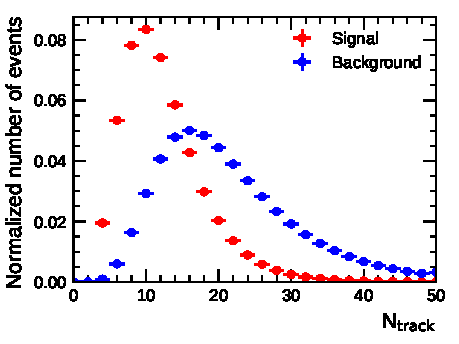
\includegraphics{./figures/rnn/ntrk_3p.pdf}
  \caption{Number of tracks for 3-prong taus}
  \label{fig:total_tracks_3p}
\end{figure}

\begin{figure}[htpb]
  \centering
  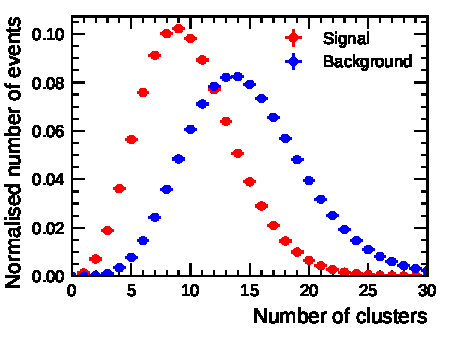
\includegraphics{./figures/rnn/ncls_3p.pdf}
  \caption{Number of clusters for 3-prong taus}
  \label{fig:total_clusters_3p}
\end{figure}

\section{MC Dijet Slices}
Truth $p_\mathrm{T}$ of jet given by anti-$k_\mathrm{T}$ jet algorithm with distance parameter $R=0.6$:
\begin{itemize}
\item[JZ0W] 0 - 20 GeV
\item[JZ1W] 20 - 60 GeV
\item[JZ2W] 60 - 160 GeV
\item[JZ3W] 160 - 400 GeV
\item[JZ4W] 400 - 800 GeV
\item[JZ5W] 800 - 1300 GeV
\item[JZ6W] 1300 - 1800 GeV
\item[JZ7W] 1800 - 2500 GeV
\item[JZ8W] 2500 - 3200 GeV
\end{itemize}

\url{https://svnweb.cern.ch/cern/wsvn/atlasoff/Generators/MC15JobOptions/trunk/share/DSID361xxx/MC15.361021.Pythia8EvtGen_A14NNPDF23LO_jetjet_JZ1W.py}


\url{https://svnweb.cern.ch/cern/wsvn/atlasoff/Generators/MC15JobOptions/trunk/common/Filters/JetFilterAkt6.py}


\url{https://svnweb.cern.ch/cern/wsvn/atlasoff/Generators/MC15JobOptions/trunk/common/Filters/JetFilter_JZX_Fragment.py}

\todo[inline]{Why is JZ0W not used}

\subsection{Preproduction Taus}
\label{app:preprod_taus}

\begin{lstlisting}[basicstyle=\small\ttfamily, breaklines=true]
  mc16_13TeV.425200.Pythia8EvtGen_A14NNPDF23LO_Gammatautau_MassWeight.merge.AOD.e5468_s2997_r9064_r8996
\end{lstlisting}

19974000 events

\subsection{MC16A Taus}
\label{app:mc16a_taus}

\begin{lstlisting}[basicstyle=\small\ttfamily, breaklines=true]
  mc16_13TeV.425200.Pythia8EvtGen_A14NNPDF23LO_Gammatautau_MassWeight.merge.AOD.e5468_s3126_r9364_r9315
\end{lstlisting}

29998000 events

\subsection{Preproduction Dijets}
\label{app:preprod_dijets}
For the tau identification studies the momentum slices (JZ1W to JZ6W) are
combined without cross section weighting as the sizes of the generated slices
are chosen such that high momentum candidates are enhanced. A cross section
reweighting would significantly reduce the weights of high momentum slices with
a large number of simulated events compared to the low momentum slices (JZ1W -
JZ2W) where only a small number of events are simulated.

\begin{lstlisting}[basicstyle=\small\ttfamily, breaklines=true]
  mc16_13TeV.361021.Pythia8EvtGen_A14NNPDF23LO_jetjet_JZ1W.merge.AOD.e3569_s2997_r9064_r8996
  mc16_13TeV.361022.Pythia8EvtGen_A14NNPDF23LO_jetjet_JZ2W.merge.AOD.e3668_s2997_r9064_r9078
  mc16_13TeV.361023.Pythia8EvtGen_A14NNPDF23LO_jetjet_JZ3W.merge.AOD.e3668_s2997_r9064_r8996
  mc16_13TeV.361024.Pythia8EvtGen_A14NNPDF23LO_jetjet_JZ4W.merge.AOD.e3668_s2997_r9064_r9078
  mc16_13TeV.361025.Pythia8EvtGen_A14NNPDF23LO_jetjet_JZ5W.merge.AOD.e3668_s2997_r9064_r8996
  mc16_13TeV.361026.Pythia8EvtGen_A14NNPDF23LO_jetjet_JZ6W.merge.AOD.e3569_s2997_r9064_r9078
\end{lstlisting}

JZ1W: 2020000 events \\
JZ2W: 1994000 events \\
JZ3W: 7801500 events \\
JZ4W: 7973500 events \\
JZ5W: 7948500 events \\
JZ6W: 1981000 events \\

\subsection{Upgrade Samples}
Gammatautau (extended layout \cite{itk_layout_slides}):
\begin{lstlisting}[basicstyle=\small\ttfamily, breaklines=true]
  mc15_14TeV.361247.PowhegPythia8EvtGen_AZNLOCTEQ6L1_Ztautau_new.recon.AOD.e4805_s2987_s2999_r8820
  mc15_14TeV.301040.PowhegPythia8EvtGen_AZNLOCTEQ6L1_DYtautau_120M180.recon.AOD.e5323_s2987_s2999_r8820
  mc15_14TeV.301041.PowhegPythia8EvtGen_AZNLOCTEQ6L1_DYtautau_180M250.recon.AOD.e5323_s2987_s2999_r8820
  mc15_14TeV.301042.PowhegPythia8EvtGen_AZNLOCTEQ6L1_DYtautau_250M400.recon.AOD.e5323_s2987_s2999_r8820
  mc15_14TeV.301043.PowhegPythia8EvtGen_AZNLOCTEQ6L1_DYtautau_400M600.recon.AOD.e5323_s2987_s2999_r8820
  mc15_14TeV.301044.PowhegPythia8EvtGen_AZNLOCTEQ6L1_DYtautau_600M800.recon.AOD.e5323_s2987_s2999_r8820
  mc15_14TeV.301045.PowhegPythia8EvtGen_AZNLOCTEQ6L1_DYtautau_800M1000.recon.AOD.e5323_s2987_s2999_r8820
  mc15_14TeV.301046.PowhegPythia8EvtGen_AZNLOCTEQ6L1_DYtautau_1000M1250.recon.AOD.e5323_s2987_s2999_r8820
  mc15_14TeV.301047.PowhegPythia8EvtGen_AZNLOCTEQ6L1_DYtautau_1250M1500.recon.AOD.e5323_s2987_s2999_r8820
  mc15_14TeV.301048.PowhegPythia8EvtGen_AZNLOCTEQ6L1_DYtautau_1500M1750.recon.AOD.e5323_s2987_s2999_r8820
  mc15_14TeV.301049.PowhegPythia8EvtGen_AZNLOCTEQ6L1_DYtautau_1750M2000.recon.AOD.e5323_s2987_s2999_r8820
  mc15_14TeV.301050.PowhegPythia8EvtGen_AZNLOCTEQ6L1_DYtautau_2000M2250.recon.AOD.e5323_s2987_s2999_r8820
  mc15_14TeV.301051.PowhegPythia8EvtGen_AZNLOCTEQ6L1_DYtautau_2250M2500.recon.AOD.e5323_s2987_s2999_r8820
  mc15_14TeV.301052.PowhegPythia8EvtGen_AZNLOCTEQ6L1_DYtautau_2500M2750.recon.AOD.e5323_s2987_s2999_r8820
  mc15_14TeV.301053.PowhegPythia8EvtGen_AZNLOCTEQ6L1_DYtautau_2750M3000.recon.AOD.e5323_s2987_s2999_r8820
  mc15_14TeV.301054.PowhegPythia8EvtGen_AZNLOCTEQ6L1_DYtautau_3000M3500.recon.AOD.e5323_s2987_s2999_r8820
  mc15_14TeV.301055.PowhegPythia8EvtGen_AZNLOCTEQ6L1_DYtautau_3500M4000.recon.AOD.e5323_s2987_s2999_r8820
  mc15_14TeV.301056.PowhegPythia8EvtGen_AZNLOCTEQ6L1_DYtautau_4000M4500.recon.AOD.e5323_s2987_s2999_r8820
  mc15_14TeV.301057.PowhegPythia8EvtGen_AZNLOCTEQ6L1_DYtautau_4500M5000.recon.AOD.e5323_s2987_s2999_r8820
  mc15_14TeV.301058.PowhegPythia8EvtGen_AZNLOCTEQ6L1_DYtautau_5000M.recon.AOD.e5323_s2987_s2999_r8820
\end{lstlisting}

Ztautau: 300000
120M180: 150000\\
180M250: 150000\\
250M400: 150000\\
400M600: 147300\\
600M800: 50000\\
800M1000: 50000\\
1000M1250: 50000\\
1250M1500: 50000\\
1500M1750: 49900\\
1750M2000: 50000\\
2000M2250: 49900\\
2250M2500: 50000\\
2500M2750: 50000\\
2750M3000: 50000\\
3000M3500: 50000\\
3500M4000: 50000\\
4000M4500: 50000\\
4500M5000: 50000\\
5000M: 49900

Dijets (extended layout):
\begin{lstlisting}[basicstyle=\small\ttfamily, breaklines=true]
  mc15_14TeV.147910.Pythia8_AU2CT10_jetjet_JZ0W.recon.AOD.e2403_s2987_s2999_r8820
  mc15_14TeV.147911.Pythia8_AU2CT10_jetjet_JZ1W.recon.AOD.e2403_s2987_s2999_r8820
  mc15_14TeV.147912.Pythia8_AU2CT10_jetjet_JZ2W.recon.AOD.e2403_s2987_s2999_r8820
  mc15_14TeV.147913.Pythia8_AU2CT10_jetjet_JZ3W.recon.AOD.e2403_s2987_s2999_r8820
  mc15_14TeV.147914.Pythia8_AU2CT10_jetjet_JZ4W.recon.AOD.e2403_s2987_s2999_r8820
  mc15_14TeV.147915.Pythia8_AU2CT10_jetjet_JZ5W.recon.AOD.e2403_s2987_s2999_r8820
  mc15_14TeV.147916.Pythia8_AU2CT10_jetjet_JZ6W.recon.AOD.e2403_s2987_s2999_r8820
  mc15_14TeV.147917.Pythia8_AU2CT10_jetjet_JZ7W.recon.AOD.e2403_s2987_s2999_r8820
\end{lstlisting}

JZ0W:999500\\
JZ1W:962300\\
JZ2W:999500\\
JZ3W:985400\\
JZ4W:50000\\
JZ5W:49650\\
JZ6W:50000\\
JZ7W:50000


\clearpage
\section{Tau-ID Variables}

\subsection{1-prong}
\begin{figure}[!ht]
  \begin{subfigure}{0.5\textwidth}
    \centering
    \includegraphics{./figures/baseline_bdt_vars/1p/centFrac.pdf}
  \end{subfigure}%
  \begin{subfigure}{0.5\textwidth}
    \centering
    \includegraphics{./figures/baseline_bdt_vars/1p/etOverPtLeadTrk.pdf}
  \end{subfigure}
  \begin{subfigure}{0.5\textwidth}
    \centering
    \includegraphics{./figures/baseline_bdt_vars/1p/innerTrkAvgDist.pdf}
  \end{subfigure}%
  \begin{subfigure}{0.5\textwidth}
    \centering
    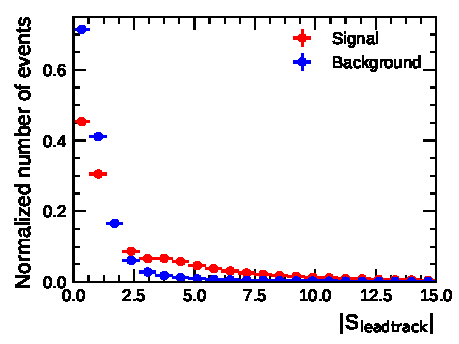
\includegraphics{./figures/baseline_bdt_vars/1p/absipSigLeadTrk.pdf}
  \end{subfigure}
  \begin{subfigure}{0.5\textwidth}
    \centering
    \includegraphics{./figures/baseline_bdt_vars/1p/SumPtTrkFrac.pdf}
  \end{subfigure}%
  \begin{subfigure}{0.5\textwidth}
    \centering
    \includegraphics{./figures/baseline_bdt_vars/1p/ChPiEMEOverCaloEME.pdf}
  \end{subfigure}
  \caption{Variables used in Tau-ID BDT. \mytodo{Rename innerTrkAvgDist x-label}}
  \label{fig:bdt_vars_1p_overlays}
\end{figure}

\begin{figure}[!ht]\ContinuedFloat
  \begin{subfigure}{0.5\textwidth}
    \centering
    \includegraphics{./figures/baseline_bdt_vars/1p/EMPOverTrkSysP.pdf}
  \end{subfigure}%
  \begin{subfigure}{0.5\textwidth}
    \centering
    \includegraphics{./figures/baseline_bdt_vars/1p/ptRatioEflowApprox.pdf}
  \end{subfigure}
  \begin{subfigure}{0.5\textwidth}
    \centering
    \includegraphics{./figures/baseline_bdt_vars/1p/mEflowApprox.pdf}
  \end{subfigure}
  \caption[]{Variables used in Tau-ID BDT}
\end{figure}

\clearpage
\subsection{3-prong}

\begin{figure}[!ht]
  \begin{subfigure}{0.5\textwidth}
    \centering
    \includegraphics{./figures/baseline_bdt_vars/3p/centFrac.pdf}
  \end{subfigure}%
  \begin{subfigure}{0.5\textwidth}
    \centering
    \includegraphics{./figures/baseline_bdt_vars/3p/etOverPtLeadTrk.pdf}
  \end{subfigure}
  \begin{subfigure}{0.5\textwidth}
    \centering
    \includegraphics{./figures/baseline_bdt_vars/3p/innerTrkAvgDist.pdf}
  \end{subfigure}%
  \begin{subfigure}{0.5\textwidth}
    \centering
    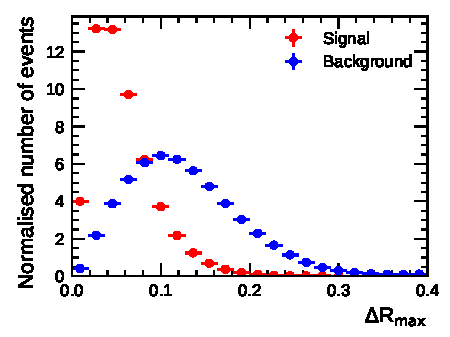
\includegraphics{./figures/baseline_bdt_vars/3p/dRmax.pdf}
  \end{subfigure}
  \begin{subfigure}{0.5\textwidth}
    \centering
    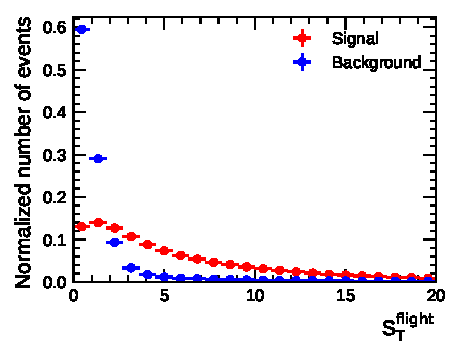
\includegraphics{./figures/baseline_bdt_vars/3p/trFlightPathSig.pdf}
  \end{subfigure}%
  \begin{subfigure}{0.5\textwidth}
    \centering
    \includegraphics{./figures/baseline_bdt_vars/3p/SumPtTrkFrac.pdf}
  \end{subfigure}%
  \caption{Variables used in Tau-ID BDT\mytodo{rename innerTrkAvgDist x-label}}
  \label{fig:bdt_vars_3p_overlays}
\end{figure}

\begin{figure}[!ht]\ContinuedFloat
  \begin{subfigure}{0.5\textwidth}
    \centering
    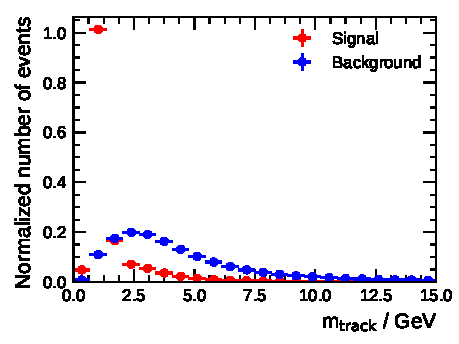
\includegraphics{./figures/baseline_bdt_vars/3p/massTrkSys.pdf}
  \end{subfigure}%
  \begin{subfigure}{0.5\textwidth}
    \centering
    \includegraphics{./figures/baseline_bdt_vars/3p/ChPiEMEOverCaloEME.pdf}
  \end{subfigure}
  \begin{subfigure}{0.5\textwidth}
    \centering
    \includegraphics{./figures/baseline_bdt_vars/3p/EMPOverTrkSysP.pdf}
  \end{subfigure}%
  \begin{subfigure}{0.5\textwidth}
    \centering
    \includegraphics{./figures/baseline_bdt_vars/3p/ptRatioEflowApprox.pdf}
  \end{subfigure}
  \begin{subfigure}{0.5\textwidth}
    \centering
    \includegraphics{./figures/baseline_bdt_vars/3p/mEflowApprox.pdf}
  \end{subfigure}
  \caption[]{Variables used in Tau-ID BDT}
\end{figure}

\clearpage
\section{Transformed Variables}
\label{app:variable_transforms}

\begin{table}[htb]
  \centering
  \begin{tabular}{ll}
  \toprule
  Variable & Transformation \\
  \midrule
  \smash{$f_\text{cent}$} & \smash{$\min(x, 1)$} \\
  \smash{$f_\text{leadtrack}^{-1}$} & \smash{$\log(\max(0.1, x))$} \\
  \smash{$R_\text{track}$} & -- \\
  \smash{$\Delta R_\text{max}$} & -- \\
  \smash{$| S_\text{leadtrack} |$} & \smash{$\min(x, 30)$} \\
  \smash{$S_\text{T}^\text{flight}$} & \smash{$\log(\max(0.01, x))$} \\
  \bottomrule
\end{tabular}\hspace*{2em}
\begin{tabular}{ll}
  \toprule
  Variable & Transformation \\
  \midrule
  \smash{$f_\text{iso}^\text{track}$} & \smash{$\log\left(x + 10^{-4}\right)$} \\
  \smash{$f_\text{EM}^\text{track-HAD}$} & \smash{$\max(-4, \min(x, 5))$} \\
  \smash{$f_\text{track}^\text{EM}$} & \smash{$\log\left(\max\left(10^{-3}, x\right)\right)$} \\
  \smash{$p_\text{T}^\text{EM+track} / p_\text{T}$} & \smash{$\min(x, 4)$} \\
  \smash{$m_\text{EM+track}$} & \smash{$\log\left(\max(140, x / \si{\MeV})\right)$} \\
  \smash{$m_\text{track}$} & \smash{$\log\left(\max(140, x / \si{MeV})\right)$} \\
  \bottomrule
\end{tabular}


%%% Local Variables:
%%% mode: latex
%%% TeX-master: "../mythesis"
%%% End:

  \caption{Transformation applied to the input variables}
\end{table}

\clearpage
\section{TMVA-BDT Configurations}
\label{app:tmva_config}

\noindent\textbf{Common for all configurations:}\\[0.3em]
\begin{tabular}{ll}
  \texttt{NegWeightTreatment} & \texttt{IgnoreNegWeightsInTraining} \\
  \texttt{PruneMethod} & \texttt{NoPruning} \\
  \texttt{SeparationType} & \texttt{GiniIndex} \\
  \texttt{UseYesNoLeaf} & \texttt{False} \\
  \texttt{nCuts} & 200
\end{tabular}

\vfill

\noindent\textbf{Old configuration:}\\[0.3em]
\begin{tabular}{ll}
  \texttt{BoostType} & \texttt{AdaBoost} \\
  \texttt{AdaBoostBeta} & 0.2 \\
  \texttt{NTrees} & 100 \\
  \texttt{MaxDepth} & 8 \\
  \texttt{MinNodeSize} & 0.1 \\
\end{tabular}

\vfill

\noindent\textbf{1-prong (Overtrained):}\\[0.3em]
\begin{tabular}{ll}
  \texttt{BoostType} & \texttt{Grad} \\
  \texttt{Shrinkage} & 0.05 \\
  \texttt{NTrees} & 800 \\
  \texttt{MaxDepth} & 16 \\
  \texttt{MinNodeSize} & 0.01 \\
\end{tabular}

\vfill

\noindent\textbf{1-prong (cool):}\\[0.3em]
\begin{tabular}{ll}
  \texttt{BoostType} & \texttt{Grad} \\
  \texttt{Shrinkage} & 0.1 \\
  \texttt{NTrees} & 400 \\
  \texttt{UseBaggedBoost} & \texttt{True} \\
  \texttt{BaggedSampleFraction} & 0.5 \\
  \texttt{MaxDepth} & 8 \\
  \texttt{MinNodeSize} & 0.1 \\
\end{tabular}

\vfill

\noindent\textbf{3-prong (Overtrained):}\\[0.3em]
\begin{tabular}{ll}
  \texttt{BoostType} & \texttt{Grad} \\
  \texttt{Shrinkage} & 0.1 \\
  \texttt{NTrees} & 800 \\
  \texttt{MaxDepth} & 16 \\
  \texttt{MinNodeSize} & 0.01 \\
\end{tabular}

\vfill

\noindent\textbf{3-prong (cool):}\\[0.3em]
\begin{tabular}{ll}
  \texttt{BoostType} & \texttt{Grad} \\
  \texttt{Shrinkage} & 0.4 \\
  \texttt{NTrees} & 800 \\
  \texttt{MaxDepth} & 6 \\
  \texttt{MinNodeSize} & 0.1 \\
\end{tabular}

\clearpage
\section{Decay Mode Classification using Recurrent Neural Networks}
\subsection{Baseline Probabilities}
\label{app:baseline_probabilities}

\begin{figure}[!ht]
  \begin{subfigure}{0.48\textwidth}
    \centering
    \includegraphics{./figures/decay_mode_classification/mode_proba_baseline_ptcut_1_5/proba_1p0n.pdf}
  \end{subfigure}\hfill
  \begin{subfigure}{0.48\textwidth}
    \centering
    \includegraphics{./figures/decay_mode_classification/mode_proba_baseline_ptcut_1_5/proba_1p1n.pdf}
  \end{subfigure}
  \begin{subfigure}{0.48\textwidth}
    \centering
    \includegraphics{./figures/decay_mode_classification/mode_proba_baseline_ptcut_1_5/proba_1pXn.pdf}
  \end{subfigure}\hfill
  \begin{subfigure}{0.48\textwidth}
    \centering
    \includegraphics{./figures/decay_mode_classification/mode_proba_baseline_ptcut_1_5/proba_3p0n.pdf}
  \end{subfigure}
  \begin{subfigure}{0.48\textwidth}
    \centering
    \includegraphics{./figures/decay_mode_classification/mode_proba_baseline_ptcut_1_5/proba_3pXn.pdf}
  \end{subfigure}%

  \caption{Multi-class probabilities for the Baseline RNN}
  \label{fig:rnn_multiclass_proba_baseline}
\end{figure}

\clearpage
\subsection{Combined Probabilities}
\label{app:combined_probabilities}

\begin{figure}[!ht]
  \begin{subfigure}{0.48\textwidth}
    \centering
    \includegraphics{./figures/decay_mode_classification/combined_proba/proba_1p0n.pdf}
  \end{subfigure}\hfill
  \begin{subfigure}{0.48\textwidth}
    \centering
    \includegraphics{./figures/decay_mode_classification/combined_proba/proba_1p1n.pdf}
  \end{subfigure}
  \begin{subfigure}{0.48\textwidth}
    \centering
    \includegraphics{./figures/decay_mode_classification/combined_proba/proba_1pXn.pdf}
  \end{subfigure}\hfill
  \begin{subfigure}{0.48\textwidth}
    \centering
    \includegraphics{./figures/decay_mode_classification/combined_proba/proba_3p0n.pdf}
  \end{subfigure}
  \begin{subfigure}{0.48\textwidth}
    \centering
    \includegraphics{./figures/decay_mode_classification/combined_proba/proba_3pXn.pdf}
  \end{subfigure}%

  \caption{Multi-class probabilities for the Combined RNN}
  \label{fig:rnn_multiclass_proba_combined}
\end{figure}

\clearpage
\section{Grid Search: 3-Prong}
\label{app:grid_search_3p}

\begin{figure}[htbp]
  \begin{subfigure}[t]{0.48\textwidth}
    \centering
    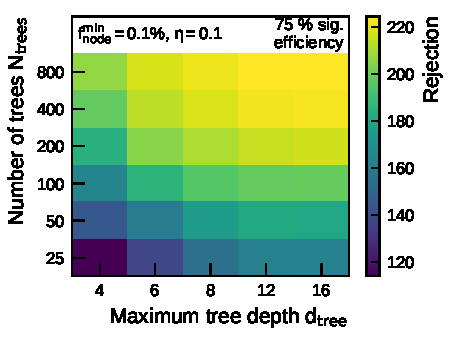
\includegraphics{./figures/bdt_perf/gridsearch_3p/scan_MaxDepth_NTrees.pdf}
    \subcaption{}
  \end{subfigure}\hfill
  \begin{subfigure}[t]{0.48\textwidth}
    \centering
    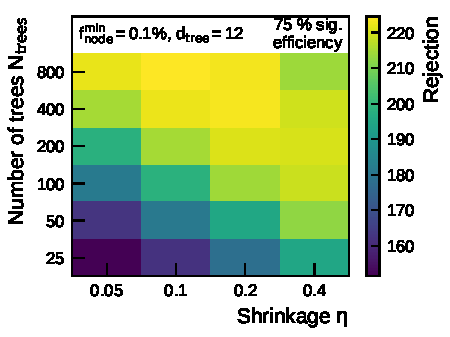
\includegraphics{./figures/bdt_perf/gridsearch_3p/scan_Shrinkage_NTrees.pdf}
    \subcaption{}
  \end{subfigure}
  \begin{subfigure}[t]{0.48\textwidth}
    \centering
    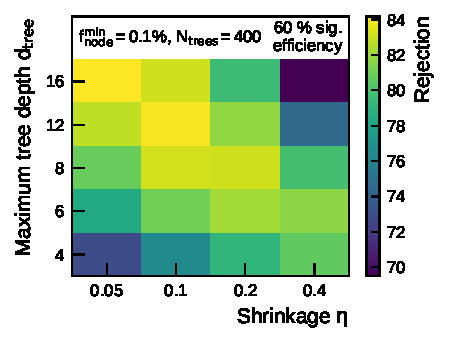
\includegraphics{./figures/bdt_perf/gridsearch_3p/scan_Shrinkage_MaxDepth.pdf}
    \subcaption{}
  \end{subfigure}\hfill
  \begin{subfigure}[t]{0.48\textwidth}
    \centering
    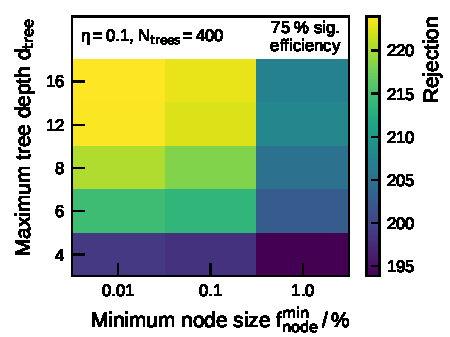
\includegraphics{./figures/bdt_perf/gridsearch_3p/scan_MinNodeSize_MaxDepth.pdf}
    \subcaption{}
  \end{subfigure}
  \caption{Background rejection at \SI{60}{\percent} signal efficiency as a
    function of the BDT hyperparameters. Bagged boosting with a subsample
    fraction~$f_\text{bag} = \SI{50}{\percent}$ is used and the remaining
    parameters are fixed such that the 'best' BDT is contained within the
    plots.}
  \todo[inline]{Better word for 'best' as it is not the best BDT}
  \label{fig:hyperparameter_scan_3p}
\end{figure}

\clearpage
\section{BDT: Recursive Feature Elimination}

\begin{figure}[htb]
  \centering
  \begin{subfigure}[t]{0.33\textwidth}
    \centering
    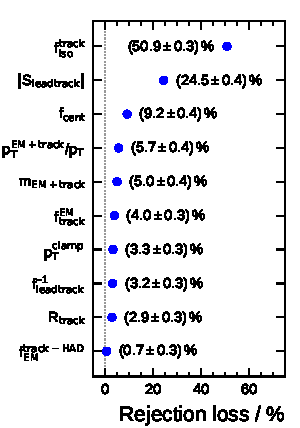
\includegraphics{./figures/bdt_perf/var_importance/1p_iter1.pdf}
    \subcaption{Iteration 1}
  \end{subfigure}
  \begin{subfigure}[t]{0.33\textwidth}
    \centering
    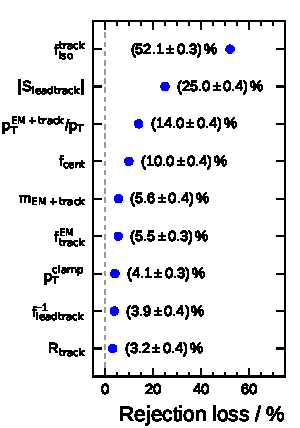
\includegraphics{./figures/bdt_perf/var_importance/1p_iter2.pdf}
    \subcaption{Iteration 2}
  \end{subfigure}
  \caption{Variable importance (1-prong). Averaged rejection loss over a
    gamma-tautau like dijet spectrum. Tight working point.}
  \label{fig:variable_importance_1p_app}
\end{figure}

\begin{figure}[htb]
  \centering
  \begin{subfigure}[t]{0.32\textwidth}
    \centering
    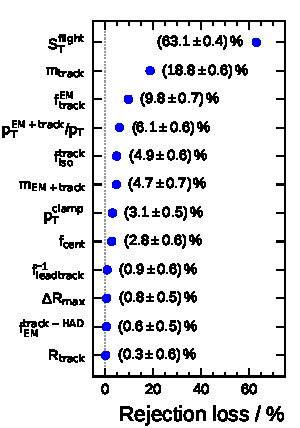
\includegraphics{./figures/bdt_perf/var_importance/3p_iter1.pdf}
    \subcaption{Iteration 1}
  \end{subfigure}
  \begin{subfigure}[t]{0.32\textwidth}
    \centering
    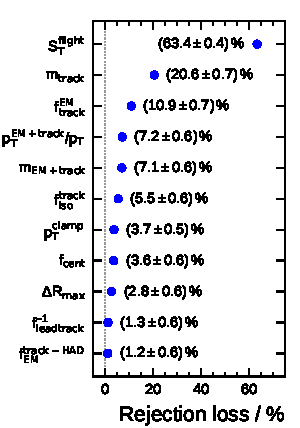
\includegraphics{./figures/bdt_perf/var_importance/3p_iter2.pdf}
    \subcaption{Iteration 2}
  \end{subfigure}
  \begin{subfigure}[t]{0.32\textwidth}
    \centering
    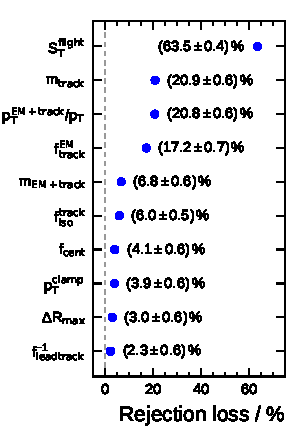
\includegraphics{./figures/bdt_perf/var_importance/3p_iter3.pdf}
    \subcaption{Iteration 3}
  \end{subfigure}

  \caption{Variable importance (3-prong). Averaged rejection loss over a
    gamma-tautau like dijet spectrum. Tight working point.}
  \label{fig:variable_importance_3p_app}
\end{figure}

\clearpage
\section{Post-Optimisation Working Points}

\begin{figure}[htb]
  \centering
  \begin{subfigure}{0.48\textwidth}
    \centering
    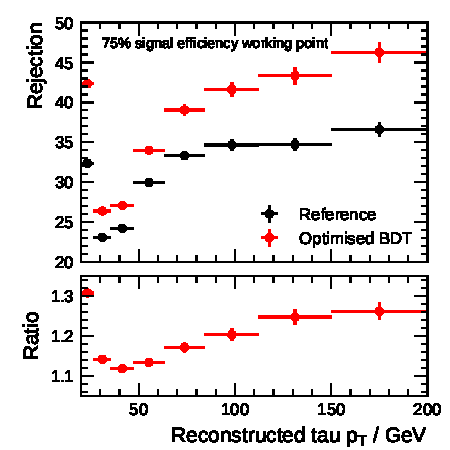
\includegraphics{./figures/bdt_perf/post_optimisation/rejection_medium_1p.pdf}
  \end{subfigure}\hfill
  \begin{subfigure}{0.48\textwidth}
    \centering
    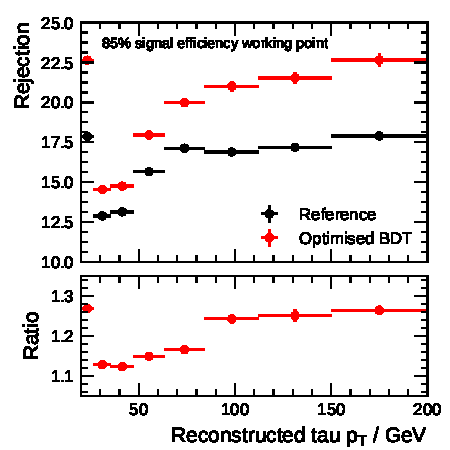
\includegraphics{./figures/bdt_perf/post_optimisation/rejection_loose_1p.pdf}
  \end{subfigure}
  \caption{1-prong}
\end{figure}

\begin{figure}[htb]
  \centering
  \begin{subfigure}{0.48\textwidth}
    \centering
    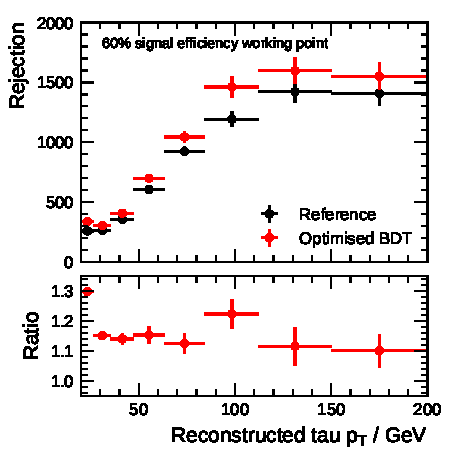
\includegraphics{./figures/bdt_perf/post_optimisation/rejection_medium_3p.pdf}
  \end{subfigure}\hfill
  \begin{subfigure}{0.48\textwidth}
    \centering
    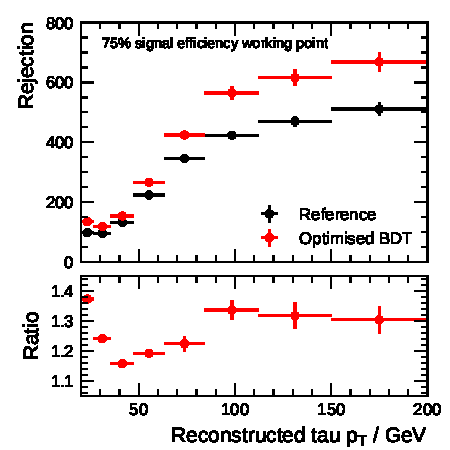
\includegraphics{./figures/bdt_perf/post_optimisation/rejection_loose_3p.pdf}
  \end{subfigure}
  \caption{3-prong}
\end{figure}

\clearpage
\section{Rejection vs.\ Initiating Parton}
\begin{figure}[htb]
  \centering
  \begin{subfigure}[t]{0.48\textwidth}
    \centering
    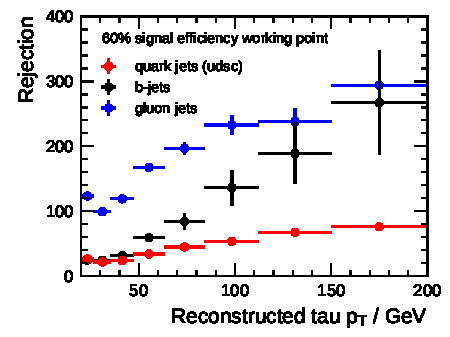
\includegraphics{./figures/bdt_perf/parton/truth_parton_1p.pdf}
    \caption{1-prong}
  \end{subfigure}\hfill
  \begin{subfigure}[t]{0.48\textwidth}
    \centering
    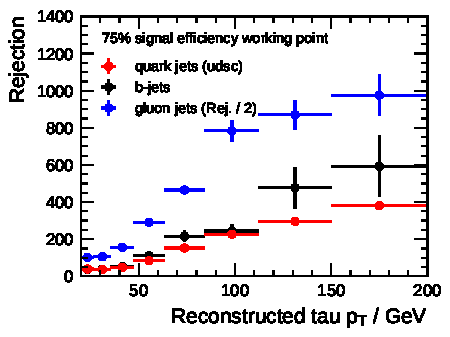
\includegraphics{./figures/bdt_perf/parton/truth_parton_3p.pdf}
    \caption{3-prong. Loose working point (Tight has too much rejection for
      limited stats)}
  \end{subfigure}
  \caption{Rejection vs initiating parton}
\end{figure}

\todo[inline]{Due to the longer decay chain of B-hadrons, the number of
  particles and angular spread is larger for a b-jet than a light-quark jet.}

\clearpage
\section{Decay Mode Classification Experiments}
\label{sec:app_decay_mode_exp}
\begin{figure}[htb]
  \begin{subfigure}[t]{0.48\textwidth}
    \centering
    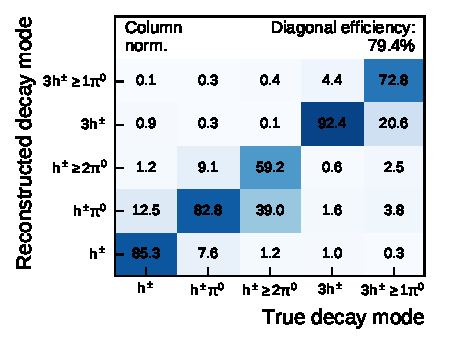
\includegraphics{./figures/decay_mode_classification/experiments/mig_mat_conversions.pdf}
    \subcaption{Migration matrix}
  \end{subfigure}\hfill
  \begin{subfigure}[t]{0.48\textwidth}
    \centering
    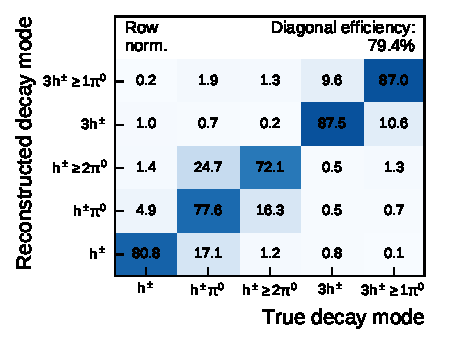
\includegraphics{./figures/decay_mode_classification/experiments/comp_mat_conversions.pdf}
    \subcaption{Composition matrix}
  \end{subfigure}
  \caption{Conversion tracks}
\end{figure}

\begin{figure}[htb]
  \begin{subfigure}[t]{0.48\textwidth}
    \centering
    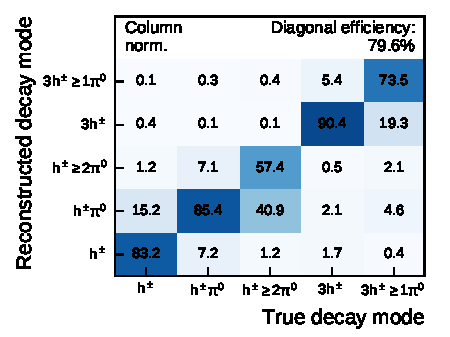
\includegraphics{./figures/decay_mode_classification/experiments/mig_mat_shots.pdf}
    \subcaption{Migration matrix}
  \end{subfigure}\hfill
  \begin{subfigure}[t]{0.48\textwidth}
    \centering
    \includegraphics{./figures/decay_mode_classification/experiments/comp_mat_shots.pdf}
    \subcaption{Composition matrix}
  \end{subfigure}
  \caption{Shots}
\end{figure}

\begin{figure}[htb]
  \begin{subfigure}[t]{0.48\textwidth}
    \centering
    \includegraphics{./figures/decay_mode_classification/experiments/mig_mat_moments.pdf}
    \subcaption{Migration matrix}
  \end{subfigure}\hfill
  \begin{subfigure}[t]{0.48\textwidth}
    \centering
    \includegraphics{./figures/decay_mode_classification/experiments/comp_mat_moments.pdf}
    \subcaption{Composition matrix}
  \end{subfigure}
  \caption{Add.\ cluster moments}
\end{figure}

\begin{figure}[htb]
  \begin{subfigure}[t]{0.48\textwidth}
    \centering
    \includegraphics{./figures/decay_mode_classification/experiments/mig_mat_hadronic_pfos.pdf}
    \subcaption{Migration matrix}
  \end{subfigure}\hfill
  \begin{subfigure}[t]{0.48\textwidth}
    \centering
    \includegraphics{./figures/decay_mode_classification/experiments/comp_mat_hadronic_pfos.pdf}
    \subcaption{Composition matrix}
  \end{subfigure}
  \caption{Hadronic PFOs}
\end{figure}

\begin{figure}[htb]
  \begin{subfigure}[t]{0.48\textwidth}
    \centering
    \includegraphics{./figures/decay_mode_classification/experiments/mig_mat_sub_e_2.pdf}
    \subcaption{Migration matrix}
  \end{subfigure}\hfill
  \begin{subfigure}[t]{0.48\textwidth}
    \centering
    \includegraphics{./figures/decay_mode_classification/experiments/comp_mat_sub_e_2.pdf}
    \subcaption{Composition matrix}
  \end{subfigure}
  \caption{$p_\text{T}$-fraction}
\end{figure}

\clearpage
\section{Combined After Tau-ID}

\begin{figure}[htbp]
  \begin{subfigure}{0.48\textwidth}
    \centering
    \includegraphics{./figures/decay_mode_classification/combined_sub_e_moments_shots_conv_ptcut_1_5/mig_mat_med_id.pdf}
    \subcaption{Migration matrix}
  \end{subfigure}\hfill
  \begin{subfigure}{0.48\textwidth}
    \centering
    \includegraphics{./figures/decay_mode_classification/combined_sub_e_moments_shots_conv_ptcut_1_5/comp_mat_med_id.pdf}
    \subcaption{ Purity matrix}
  \end{subfigure}
  \caption{Combined with medium tau id}
  \label{fig:decay_mode_combined_med_id}
\end{figure}

\clearpage
\section{Track-Constrained Decay Mode Classification}
\label{app:mode_classification_track_constraint}

\begin{figure}[htbp]
  \begin{subfigure}{0.48\textwidth}
    \centering
    \includegraphics{./figures/decay_mode_classification/combined_sub_e_moments_shots_conv_ptcut_1_5/mig_mat.pdf}
    \subcaption{Extended model without track constraint.}
  \end{subfigure}\hfill
  \begin{subfigure}{0.48\textwidth}
    \centering
    \includegraphics{./figures/decay_mode_classification/combined_sub_e_moments_shots_conv_ptcut_1_5/mig_mat_use_ntracks.pdf}
    \subcaption{Extended model with track constraint.}
  \end{subfigure}
  \caption{Migration matrix for the extended model including conversion, shot
    and additional cluster information. The model is constrained by setting
    estimated mode probabilities to zero for modes not consistent with the
    number of reconstructed tracks.}
\end{figure}

\clearpage
\section{High-$p_\text{T}$}
\label{sec:combined_high_pt_migration}

\begin{figure}[htb]
    \begin{subfigure}{0.48\textwidth}
    \centering
    \includegraphics{./figures/decay_mode_classification/highpt/mig_mat_pt_less_100.pdf}
    \subcaption{Migration matrix. $p_\text{T} < \SI{100}{\giga\electronvolt}$}
  \end{subfigure}\hfill
  \begin{subfigure}{0.48\textwidth}
    \centering
    \includegraphics{./figures/decay_mode_classification/highpt/comp_mat_pt_less_100.pdf}
    \subcaption{Migration matrix. $p_\text{T} < \SI{100}{\giga\electronvolt}$}
  \end{subfigure}
  \begin{subfigure}{0.48\textwidth}
    \centering
    \includegraphics{./figures/decay_mode_classification/highpt/mig_mat_pt_geq_100.pdf}
    \subcaption{Migration matrix. $p_\text{T} > \SI{100}{\giga\electronvolt}$}
  \end{subfigure}\hfill
  \begin{subfigure}{0.48\textwidth}
    \centering
    \includegraphics{./figures/decay_mode_classification/highpt/comp_mat_geq_100.pdf}
    \subcaption{Purity matrix. $p_\text{T} > \SI{100}{\giga\electronvolt}$}
  \end{subfigure}
  \caption{highpt}
  \label{fig:highpt_matrices}
\end{figure}

\clearpage
\section{TODOS}
\listoftodos

%%% Local Variables:
%%% mode: latex
%%% TeX-master: "mythesis"
%%% End:

\printbibliography[heading=subbibliography]

%------------------------------------------------------------------------------
% Declare lists of figures and tables and acknowledgements as backmatter
% Chapter/section numbers are turned off
\backmatter

\listoffigures
\listoftables

%------------------------------------------------------------------------------
% Print the glossary and list of acronyms
% \printglossaries

%------------------------------------------------------------------------------
% You could instead add your acknowledgements here - don't forget to
% also add them to \includeonly above
% %------------------------------------------------------------------------------
\chapter{Acknowledgements}
\label{sec:ack}
%------------------------------------------------------------------------------

This thesis would not have been possible without the help, guidance and support
of many people. Therefore, I would like to thank:
\begin{itemize}
\item Prof.\ Dr.\ Jochen Dingfelder for giving me the opportunity to write my
  thesis in his working group and for his continued support.

\item Prof.\ Dr.\ Klaus Desch for his willingness to co-examine my thesis.

\item Dr.\ William Davey for his excellent supervision, guidance and the many
  fruitful discussions.

\item Benedict Winter for his valuable advice and him sharing his vast
  knowledge of physics with me.

\item My (past) office colleagues Verena Muckhoff, Jan Heinrichs, and Christos
  Vergis for the enjoyable office atmosphere.

\item All of my colleagues in the working group of Prof.\ Dingfelder.

\item My family for providing me with support and stability during my studies.

\end{itemize}



%%% Local Variables:
%%% mode: latex
%%% TeX-master: "mythesis"
%%% End:


%------------------------------------------------------------------------------
% CV needed when you submit your PhD thesis
% \definecolor{lightgray}{gray}{0.8}
\newcolumntype{L}{>{\raggedleft}p{0.15\textwidth}}
\newcolumntype{R}{p{0.8\textwidth}}
\newcommand\VRule{\color{lightgray}\vrule width 0.5pt}

\thispagestyle{empty}
\section*{Curriculum Vitae}

\subsection*{Personal Details}

\begin{tabular}{L!{\VRule}R}
Name & Johann Schmidt \\
Date of Birth &  \\
Email & abc@physik.uni-def.de \\
Family status & Single
\end{tabular}

\subsection*{Education}

\begin{tabular}{L!{\VRule}R}
1997--2003 & Abitur, ABC Secondary School, Hamburg, Germany\\
2004--2007 & BSc in Physics, Rheinische Friedrich-Wilhelms-Universität, Bonn, Germany.\\
2006 & CERN Summer Student, Geneva, Switzerland. \\
2007--2009 &  MSc in Physics Rheinische Friedrich-Wilhelms-Universität, Bonn, Germany. \\
2009--2012 &  PhD in Physics, Rheinische Friedrich-Wilhelms-Universität, Bonn, Germany. \\
2012 & Advanced Data Analysis School, Frankfurt, Germany.
\end{tabular}

\subsection*{Professional Experience}

\begin{tabular}{L!{\VRule}R}
2004 & Summer Student at CERN, Geneva, Switzerland. \\
2007--2012 & Doctoral work at the University of Bonn, Germany. \\
2008--2009 & Fieldwork at CERN, Geneva, Switzerland.\\
2011 & Talk at the Advanced Physics Conference, Timbucto
\end{tabular}

\subsection*{Languages}
\begin{tabular}{L!{\VRule}R}
German & Mother tongue \\
English & Fluent \\
Russian & Basic
\end{tabular}


\end{document}

%%% Local Variables:
%%% mode: latex
%%% TeX-master: t
%%% End:
